\documentclass[fleqn]{hermans-hw}

\usepackage{notes}
\usepackage{url}
\usepackage{graphicx}
\usepackage{tikz}
\usepackage{amsmath}
\usepackage[linewidth=1pt, leftmargin=0,rightmargin=0, innertopmargin = \topskip,splittopskip=\topskip, innerleftmargin=2,innerrightmargin=10]{mdframed}
\topmargin -1.5cm        % read Lamport p.163
\oddsidemargin -0.04cm   % read Lamport p.163
\evensidemargin -0.04cm  % same as oddsidemargin but for left-hand pages
\textwidth 16.59cm
\textheight 21.94cm
\parskip 7.2pt           % sets spacing between paragraphs


\title{HW6: Hidden Markov Models}
\class{CS6300: Artificial Intelligence, Spring 2018}
\institute{University of Utah}
\author{Jake Pitkin}
% IF YOU'RE USING THIS .TEX FILE AS A TEMPLATE, PLEASE REPLACE
% The author WITH YOUR NAME AND UID.
% Replace the due date with anyone you worked with i.e. "Worked with: John McCarthy, Watson, & Hal-9000"
\begin{document}
\maketitle
\section{Stationary Distributions of Markov Chains}

\begin{enumerate}
\item {\bf Suppose that in semester $t=0$ Alice passes the class with
  probability $0.5$.  Compute the probability that she passes in
  semester $t=1$ and semester $t=2$.}
  
We are given an initial distribution and transition matrix as follows:

$$\pi_0 = \begin{bmatrix} 0.5 & 0.5 \\ \end{bmatrix}$$

$$P = \begin{bmatrix}
 0.8 & 0.2 \\
 0.4 & 0.6
\end{bmatrix}$$

To compute the probabilities at $t = 1$ we apply matrix multiplication:

$$\pi_0 P = \pi_1 = \begin{bmatrix} 0.6 & 0.4 \\ \end{bmatrix}$$

To compute the probabilities at $t = 2$ we apply matrix multiplication again this time to $\pi_1$ and $P$:

$$\pi_0 P = \pi_1 = \begin{bmatrix} 0.64 & 0.36 \\ \end{bmatrix}$$

$$\boxed{P(t_1 = pass) = 0.6, \ \ \ P(t_2 = pass) = 0.64}$$

\item {\bf Compute the stationary distribution of this chain.  (Hint: the
  easiest way to do this is to start with some ``guess'' -- say 50/50
  -- and then keep simulating the chain for a while until it seems to
  settle down.  Once you think you've got a guess at what the
  stationary distribution might be, try transitioning from there to
  see if you get back to the stationary distribution.)  (Not as
  helpful hint: if you like linear algebra, you can directly compute
  the stationary distribution from the transition matrix using an
  eigenvalue decomposition: take a look at Wikipedia for how!)}
  
I'll use the technique of starting the distribution at $\pi_0 = [0.5 \ 0.5]$, simulating the chain for a while and waiting for it to settle down. I simulated the chain for $t = 100$ using a program and arrived at $\pi = [0.6667 \ 0.3333]$. We can verify this by transitioning and checking if we arrive at the stationary distribution:

$$\pi P = [0.6667 \ 0.3333] \begin{bmatrix}
 0.8 & 0.2 \\
 0.4 & 0.6
\end{bmatrix} = [0.6667 \ 0.3333] = \pi$$

Thus the stationary distribution is:

$$\boxed{\pi = \Big[\frac{2}{3} \ \frac{1}{3}\Big]}$$
\end{enumerate}
\vspace{-0.5cm}
\section{Alice and the Crazy Coke Machine}

\begin{enumerate}
\item {\bf Draw a state space lattice for this soda machine (as on the final slide of day 20) for three time steps. }

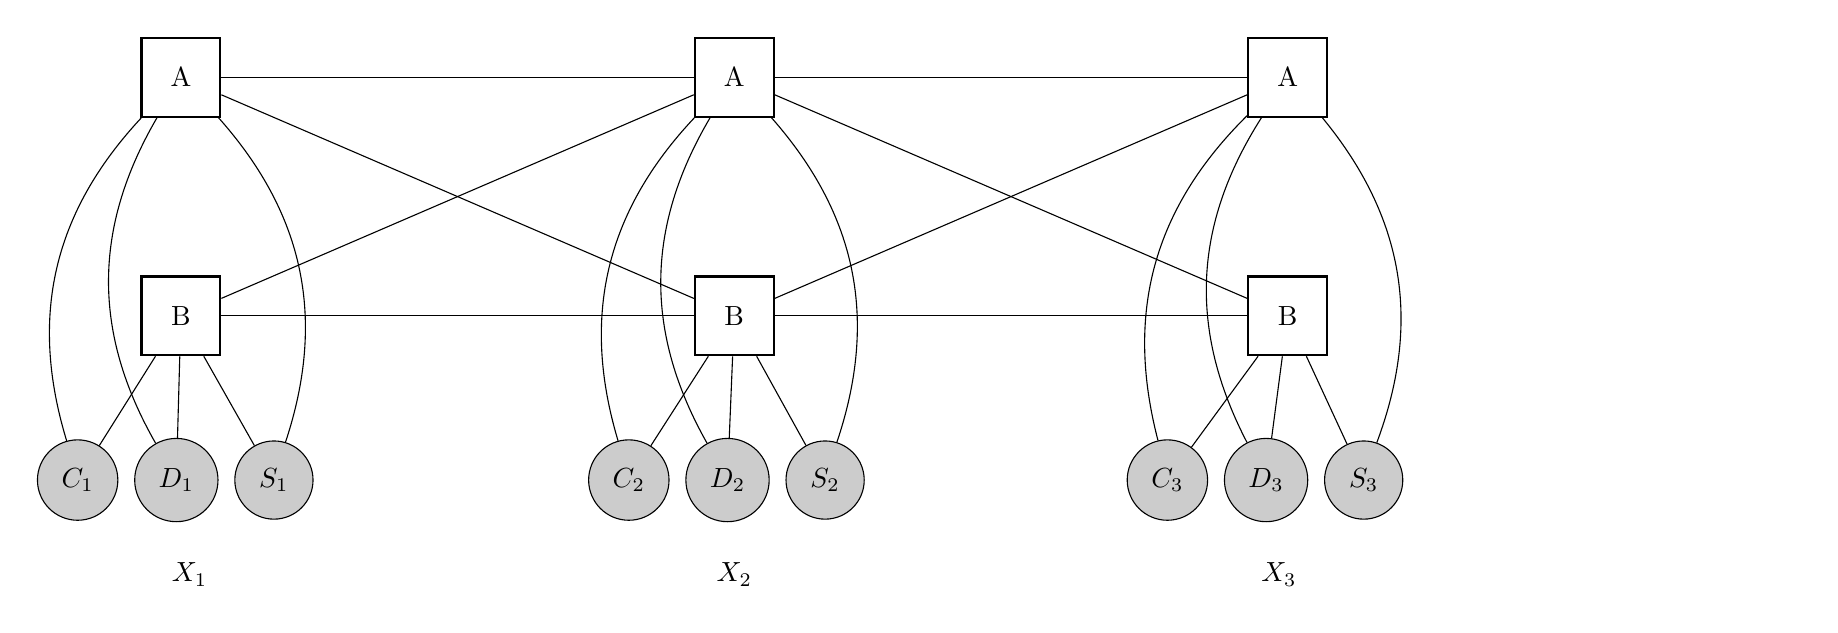
\begin{tikzpicture}[scale=2]
    \tikzstyle{ann} = [draw=none,fill=none,right]
        
    \matrix[nodes={draw, minimum size=0.1cm, fill=black!20},
        row sep=0cm,column sep=0.2cm] at (-5,-1.8){
    \node[circle] (7) {\ $C_1$ \ }; &
    \node[circle] (8) {\ $D_1$ \ }; &
    \node[circle] (9) {\ $S_1$ \ }; & \\
    };
    
    \matrix[nodes={draw , minimum size=0.1cm, fill=black!20},
        row sep=0cm,column sep=0.2cm] at (-1.5,-1.8){
    \node[circle] (10) {\ $C_2$ \ }; &
    \node[circle] (11) {\ $D_2$ \ }; &
    \node[circle] (12) {\ $S_2$ \ }; & \\
    };
    
    \matrix[nodes={draw, minimum size=0.1cm, fill=black!20},
        row sep=0cm,column sep=0.2cm] at (1.92,-1.8){
    \node[circle] (13) {\ $C_3$ \ }; &
    \node[circle] (14) {\ $D_3$ \ }; &
    \node[circle] (15) {\ $S_3$ \ }; & \\
    };
    
    \matrix[nodes={draw, thick, minimum size=1cm},
        row sep=2cm,column sep=6cm] at (0,0) {
    \node[rectangle] (1) {\ A \ }; &
    \node[rectangle] (2) {\ A \ }; &
    \node[rectangle] (3) {\ A \ }; & \\
    \node[rectangle] (4) {\ B \ }; &
    \node[rectangle] (5) {\ B \ }; &
    \node[rectangle] (6) {\ B \ }; & \\
    };
    
    \matrix[nodes={draw, thick},
        row sep=1cm,column sep=6cm] at (0, -2.4){
    \node[draw=none,fill=none] (16) {\ $X_1$ \ }; &
    \node[draw=none,fill=none] (17) {\ $X_2$ \ }; &
    \node[draw=none,fill=none] (18) {\ $X_3$ \ }; & \\
    };

    \draw[]  (1) edge node{} (2);
    \draw[]  (2) edge node{} (3);
    \draw[]  (2) edge node{} (6);
    \draw[]  (4) edge node{} (5);
    \draw[]  (5) edge node{} (6);
    \draw[]  (1) edge node{} (5);
    \draw[]  (4) edge node{} (2);
    \draw[]  (5) edge node{} (3);
    
    \draw[]  (1) edge[bend right] node{} (7);
    \draw[]  (1) edge[bend right] node{} (8);
    \draw[]  (1) edge[bend left] node{} (9);
    \draw[]  (4) edge node{} (7);
    \draw[]  (4) edge node{} (8);
    \draw[]  (4) edge node{} (9);
    
    \draw[]  (2) edge[bend right] node{} (10);
    \draw[]  (2) edge[bend right] node{} (11);
    \draw[]  (2) edge[bend left] node{} (12);
    \draw[]  (5) edge node{} (10);
    \draw[]  (5) edge node{} (11);
    \draw[]  (5) edge node{} (12);
    
    \draw[]  (3) edge[bend right] node{} (13);
    \draw[]  (3) edge[bend right] node{} (14);
    \draw[]  (3) edge[bend left] node{} (15);
    \draw[]  (6) edge node{} (13);
    \draw[]  (6) edge node{} (14);
    \draw[]  (6) edge node{} (15);


\end{tikzpicture}

Where square nodes are states and circle nodes are observations.

\item {\bf Suppose that Alice doesn't know what state the machine is in
  currently (specifically, she believes it's equally likely to be in
  either state), but puts money in and gets a Sprite out.  What is the
  probability distribution over states that it was in when Alice put
  her money in?  What is the probability distribution over states that
  it is in now?}
  
  Before Alice puts any money into the machine she believes there is a uniform distribution over possible states:
  
  $$\boxed{P(A_0) = 0.5, \ \ \ P(B_0) = 0.5}$$
  
  Now Alice puts in money and gets a Sprite. We will compute the probability of being in each state given we observed a Sprite using Bayes' rule:
  
  $$P(A_1 | S_1) = \frac{P(S_1 | A_1) P(A_1)}{P(S_1)}$$
  
  $$P(B_1 | S_1) = \frac{P(S_1 | B_1) P(B_1)}{P(S_1)}$$
  
  We know $P(S_1 | A_1) = 1/4$ and $P(S_1 | B_1)$ = $1/3$ from the problem. We must compute $P(A_1)$ and $P(B_1)$ first:
  
  $$P(A_1) = P(A_1 | A_0)P(A_0) + P(A_1 | B_0)P(B_0) = 0.8 * 0.5 + 0.4 * 0.5 = 0.6$$
  
  $$P(B_1) = P(B_1 | B_0)P(B_0) + P(B_1 | A_0)P(A_0) = 0.6 * 0.5 + 0.2 * 0.5 = 0.4$$
  
  Now that we have these, we can compute $P(S_1)$:
  
  $$P(S_1) = P(S_1 | A_1)P(A_1) + P(S_1 | B_1)P(B_1) = 0.25 * 0.6 + 0.333333 * 0.4 = 0.28333$$
  
  Putting it all together:
  
  $$P(A_1 | S_1) = \frac{P(S_1 | A_1) P(A_1)}{P(S_1)} = \frac{0.25 * 0.6}{0.28333} = 0.5294$$
  
  $$P(B_1 | S_1) = \frac{P(S_1 | B_1) P(B_1)}{P(S_1)} = \frac{0.3333 * 0.4}{0.28333} = 0.4706$$
  
  $$\boxed{P(A_1 | S_1) = 0.5294, \ \ \ P(B_1 | S_1) = 0.4706}$$

\item {\bf Suppose Alice comes back the next day (so again she doesn't know
  what state the machine is in) and really wants a diet coke.
  Unfortunately, the machine isn't being particularly nice to her and
  it produces the following series of emissions upon taking money from
  Alice: C S S D.  What is the most likely sequence of states the
  machine went through in this process?}
\end{enumerate}
\end{document}
